\documentclass{beamer}

%------------------------------------------------------------
%   BEAMER THEME AND PACKAGES
%------------------------------------------------------------
\usetheme{Madrid}
\usecolortheme{default}

\usepackage[utf8]{inputenc}
\usepackage[english]{babel}
\usepackage{amsmath}
\usepackage{graphicx}
\usepackage{url}

% --- BIBLATEX PACKAGE (for modern bibliography) ---
\usepackage[backend=biber, style=numeric]{biblatex}
\addbibresource{references.bib} % IMPORTANT: The .bib extension is required here

%------------------------------------------------------------
%   PRESENTATION INFORMATION
%------------------------------------------------------------

\title[QMD \& DFT]{A Journey into Quantum Molecular Dynamics and DFT} 
\author{Bryan Martinez Anzola \and Jose Luis Zamora \and Juan Sebastian Acuña}
\institute{Universidad Distrital Francisco José de Caldas}
\date{\today}

%------------------------------------------------------------
%   BEGIN DOCUMENT
%------------------------------------------------------------

\begin{document}

% --- TITLE PAGE ---
\begin{frame}
    \titlepage
\end{frame}

% --- TABLE OF CONTENTS ---
\begin{frame}{Outline}
    \tableofcontents
\end{frame}

%------------------------------------------------------------
%   SECTIONS
%------------------------------------------------------------

% --- SECTION 1: History of Quantum Molecular Dynamics ---
\section{History of Quantum Molecular Dynamics}
\begin{frame}{Origins of Molecular Dynamics (MD)}
    \begin{itemize}
        \item Modern MD was developed in the 1950s, influenced by Monte Carlo methods popularized at Los Alamos National Laboratory.
        \pause
        \bigskip
        \item However, interest in the evolution of N-body systems dates back to the 17th century with Isaac Newton, focusing mainly on celestial mechanics.
        \pause
        \bigskip
        \item Many key numerical algorithms were created before computers. For example, the \textbf{Verlet integration algorithm}, the most common today, was used as early as 1791 by Jean Baptiste Joseph Delambre.
    \end{itemize}
\end{frame}

\begin{frame}{Pre-Computational Methods}
    Before digital computers, modeling was done in other ways:
    \pause
    
    \begin{itemize}
        \item \textbf{Analog computers} were used to integrate the equations of motion.
        \pause
        \item Some scientists built \textbf{physical models} with spheres to replicate the structure of liquids and study their behavior.
    \end{itemize}
    \pause
    
    \begin{block}<4->{The Fermi-Pasta-Ulam-Tsingou Problem}
        To understand the origin of irreversibility, Enrico Fermi and his collaborators used the \textbf{MANIAC I} computer in 1953 to simulate the time evolution of a many-body system.
    \end{block}
\end{frame}

\begin{frame}{Los Autores del Problema FPU}
    \begin{columns}[T] % La opción [T] alinea las columnas por la parte superior
        \begin{column}{0.24\textwidth}
            \centering
            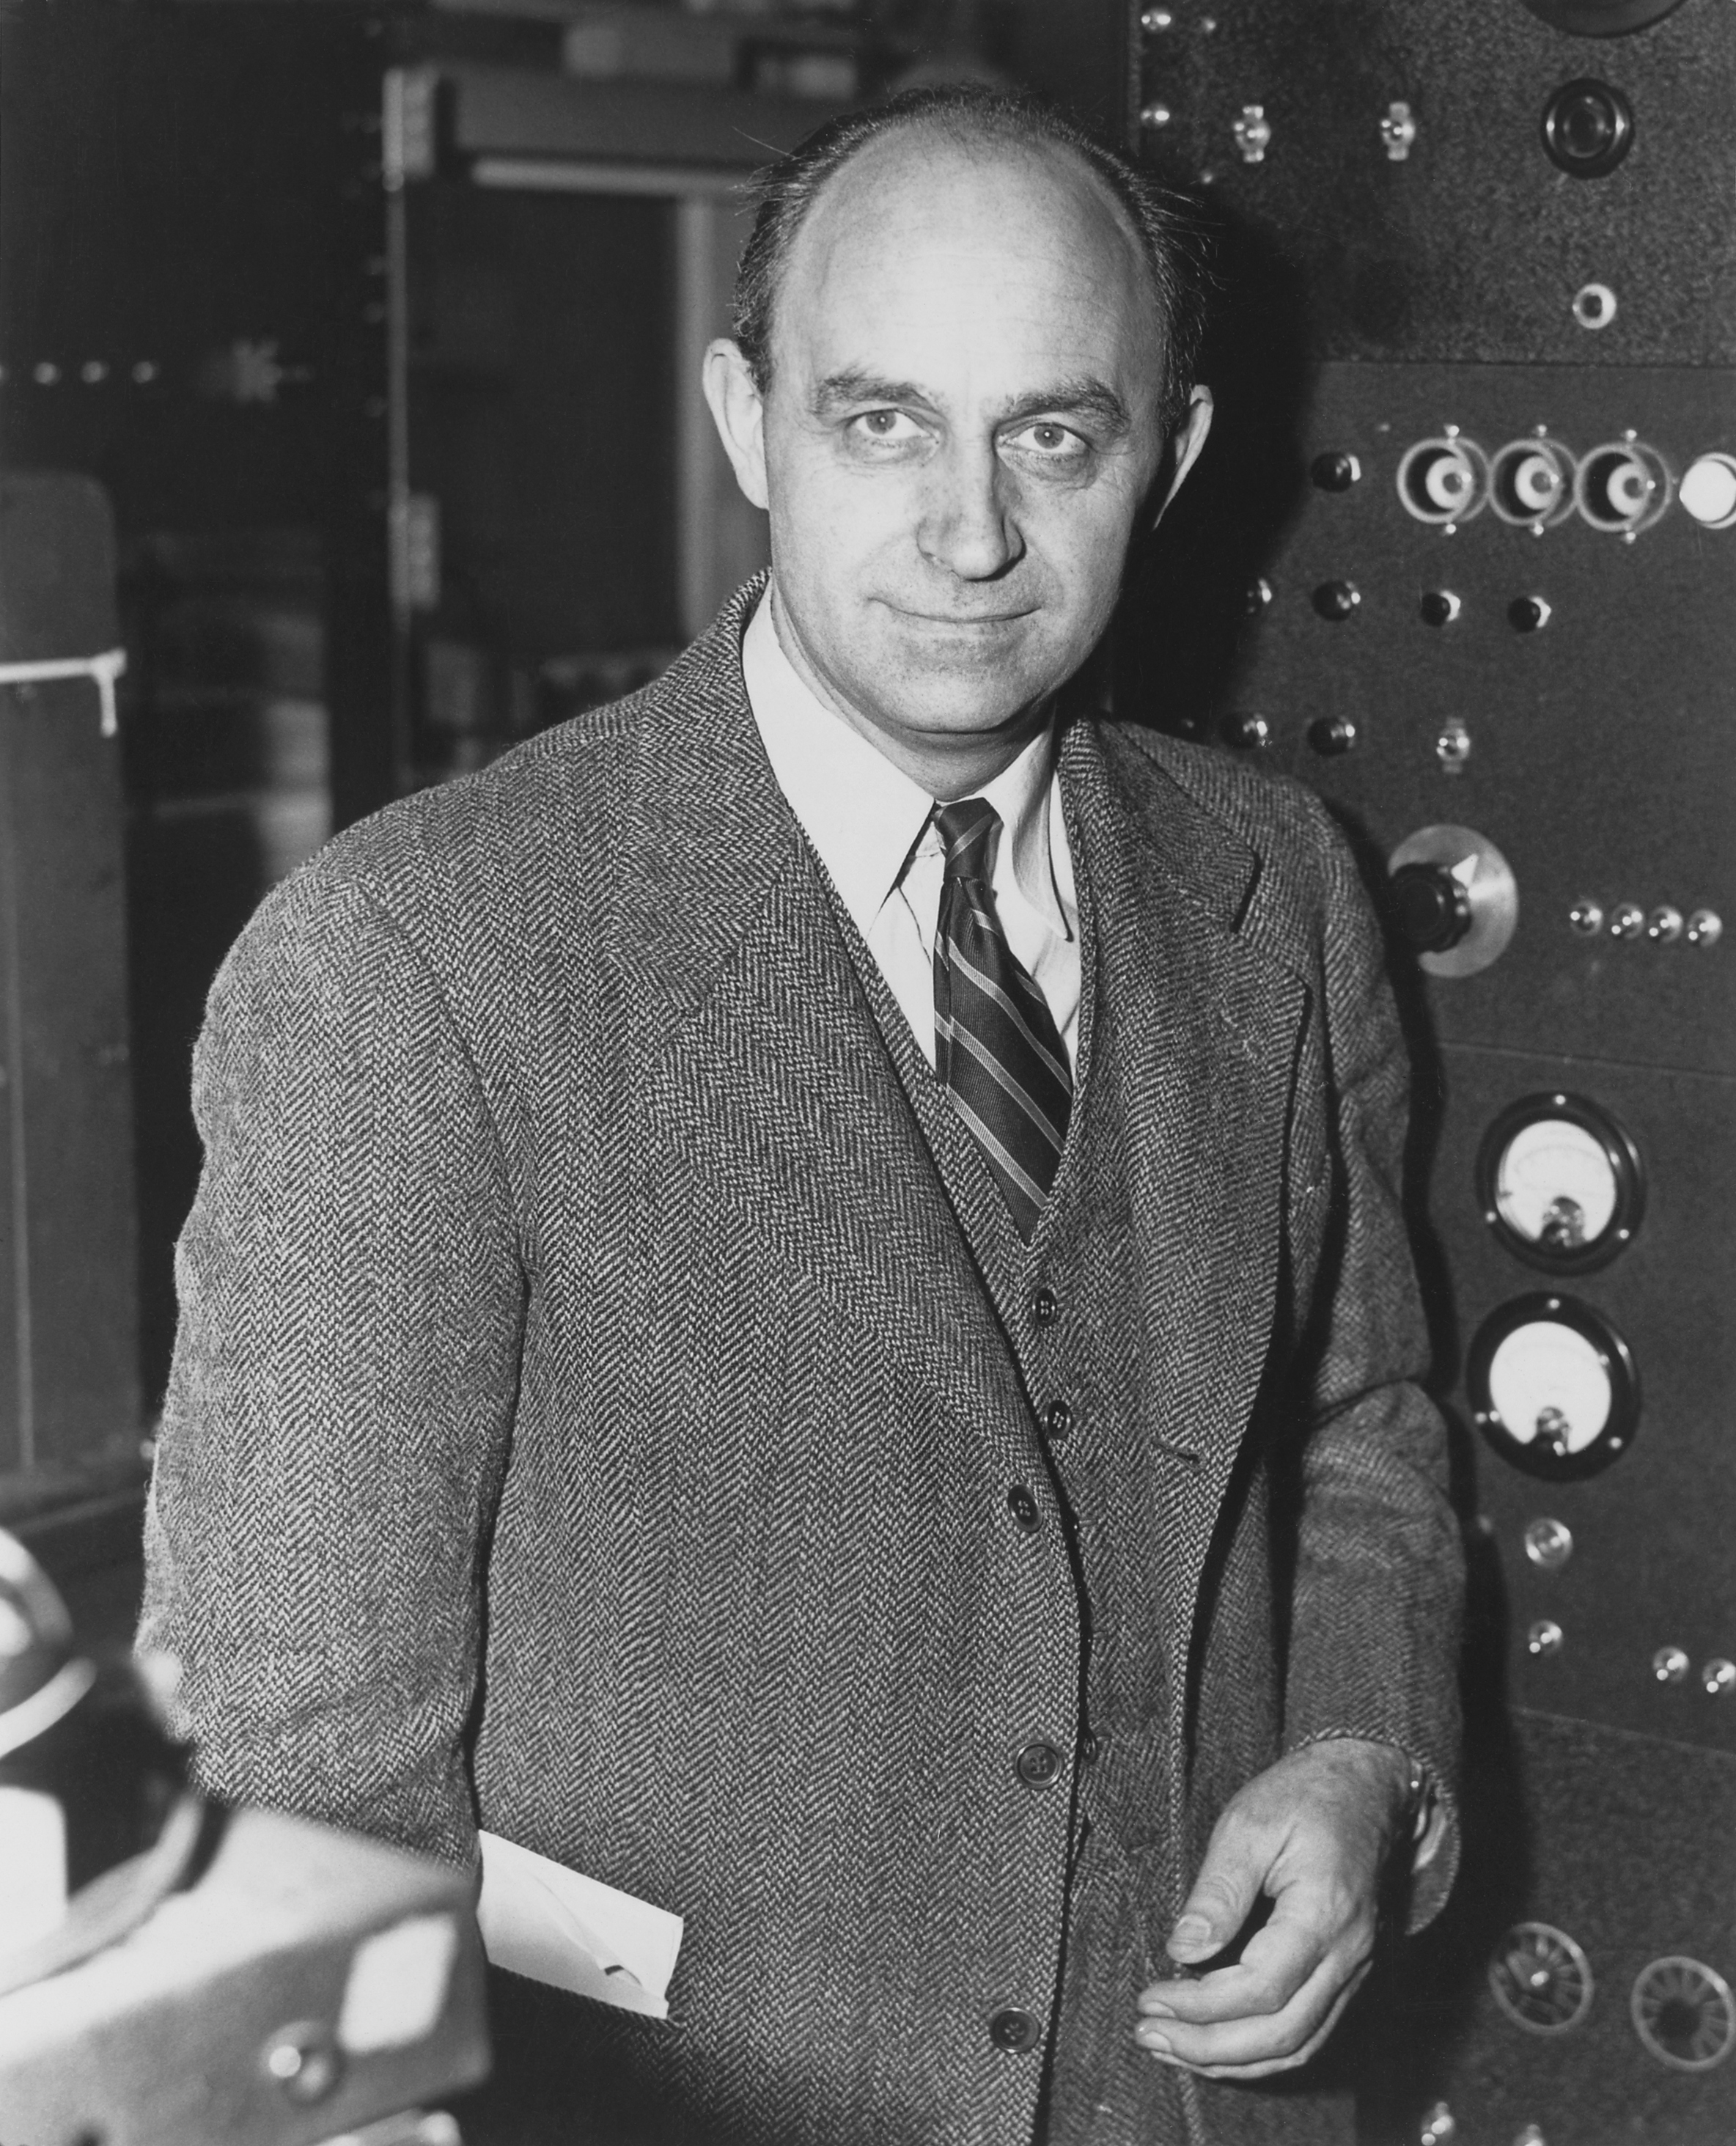
\includegraphics[width=\textwidth]{images/fermi_face.jpg}
            Enrico Fermi
        \end{column}
        
        \begin{column}{0.24\textwidth}
            \centering
            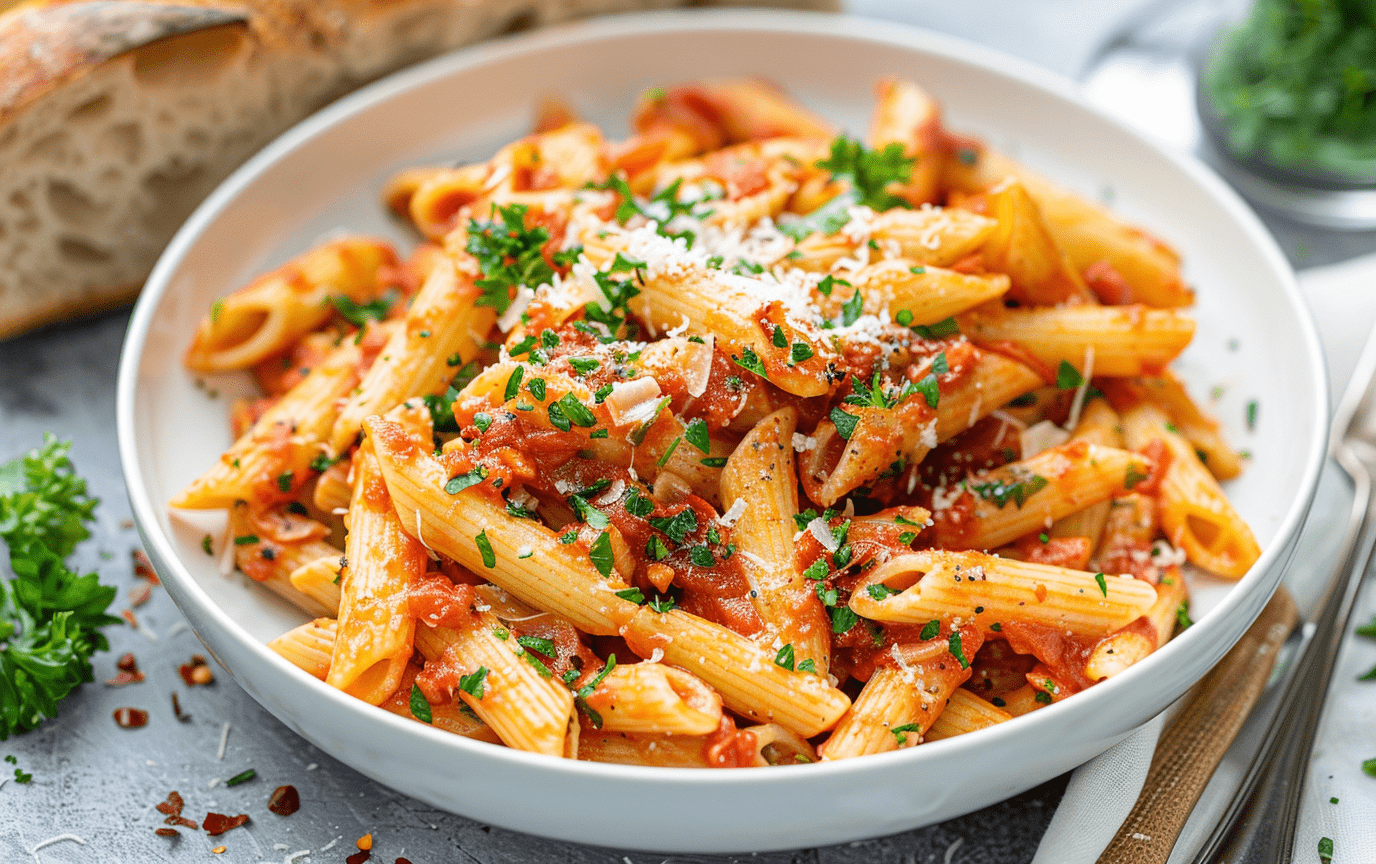
\includegraphics[width=\textwidth]{images/pasta.png}
            John Pasta
        \end{column}
        
        \begin{column}{0.24\textwidth}
            \centering
            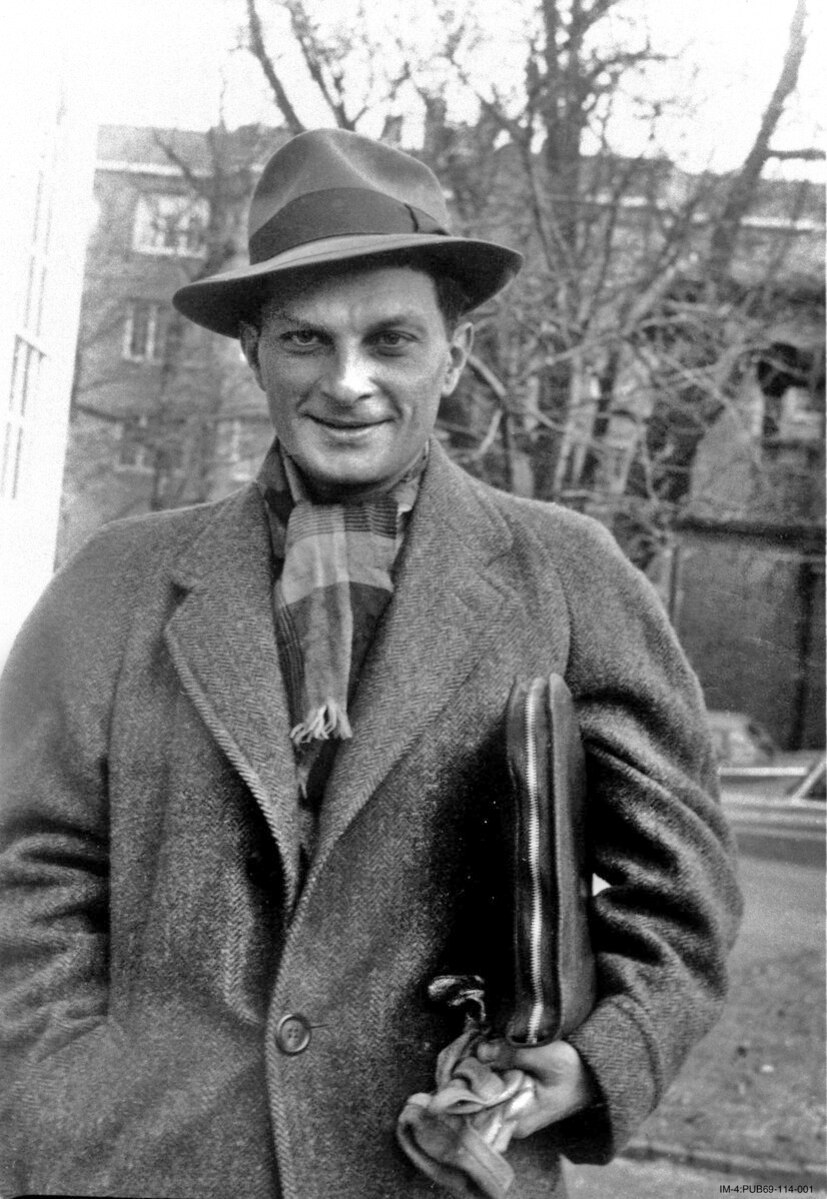
\includegraphics[width=\textwidth]{images/ulam.jpg}
            Stanislaw Ulam
        \end{column}
        
        \begin{column}{0.24\textwidth}
            \centering
            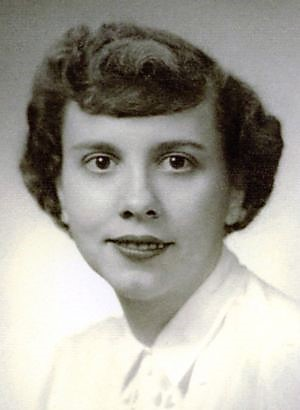
\includegraphics[width=\textwidth]{images/tsingou.jpg}
            Mary Tsingou
        \end{column}
    \end{columns}
\end{frame}

\begin{frame}{Los Autores del Problema FPU}
    \begin{columns}[T] % La opción [T] alinea las columnas por la parte superior
        \begin{column}{0.24\textwidth}
            \centering
            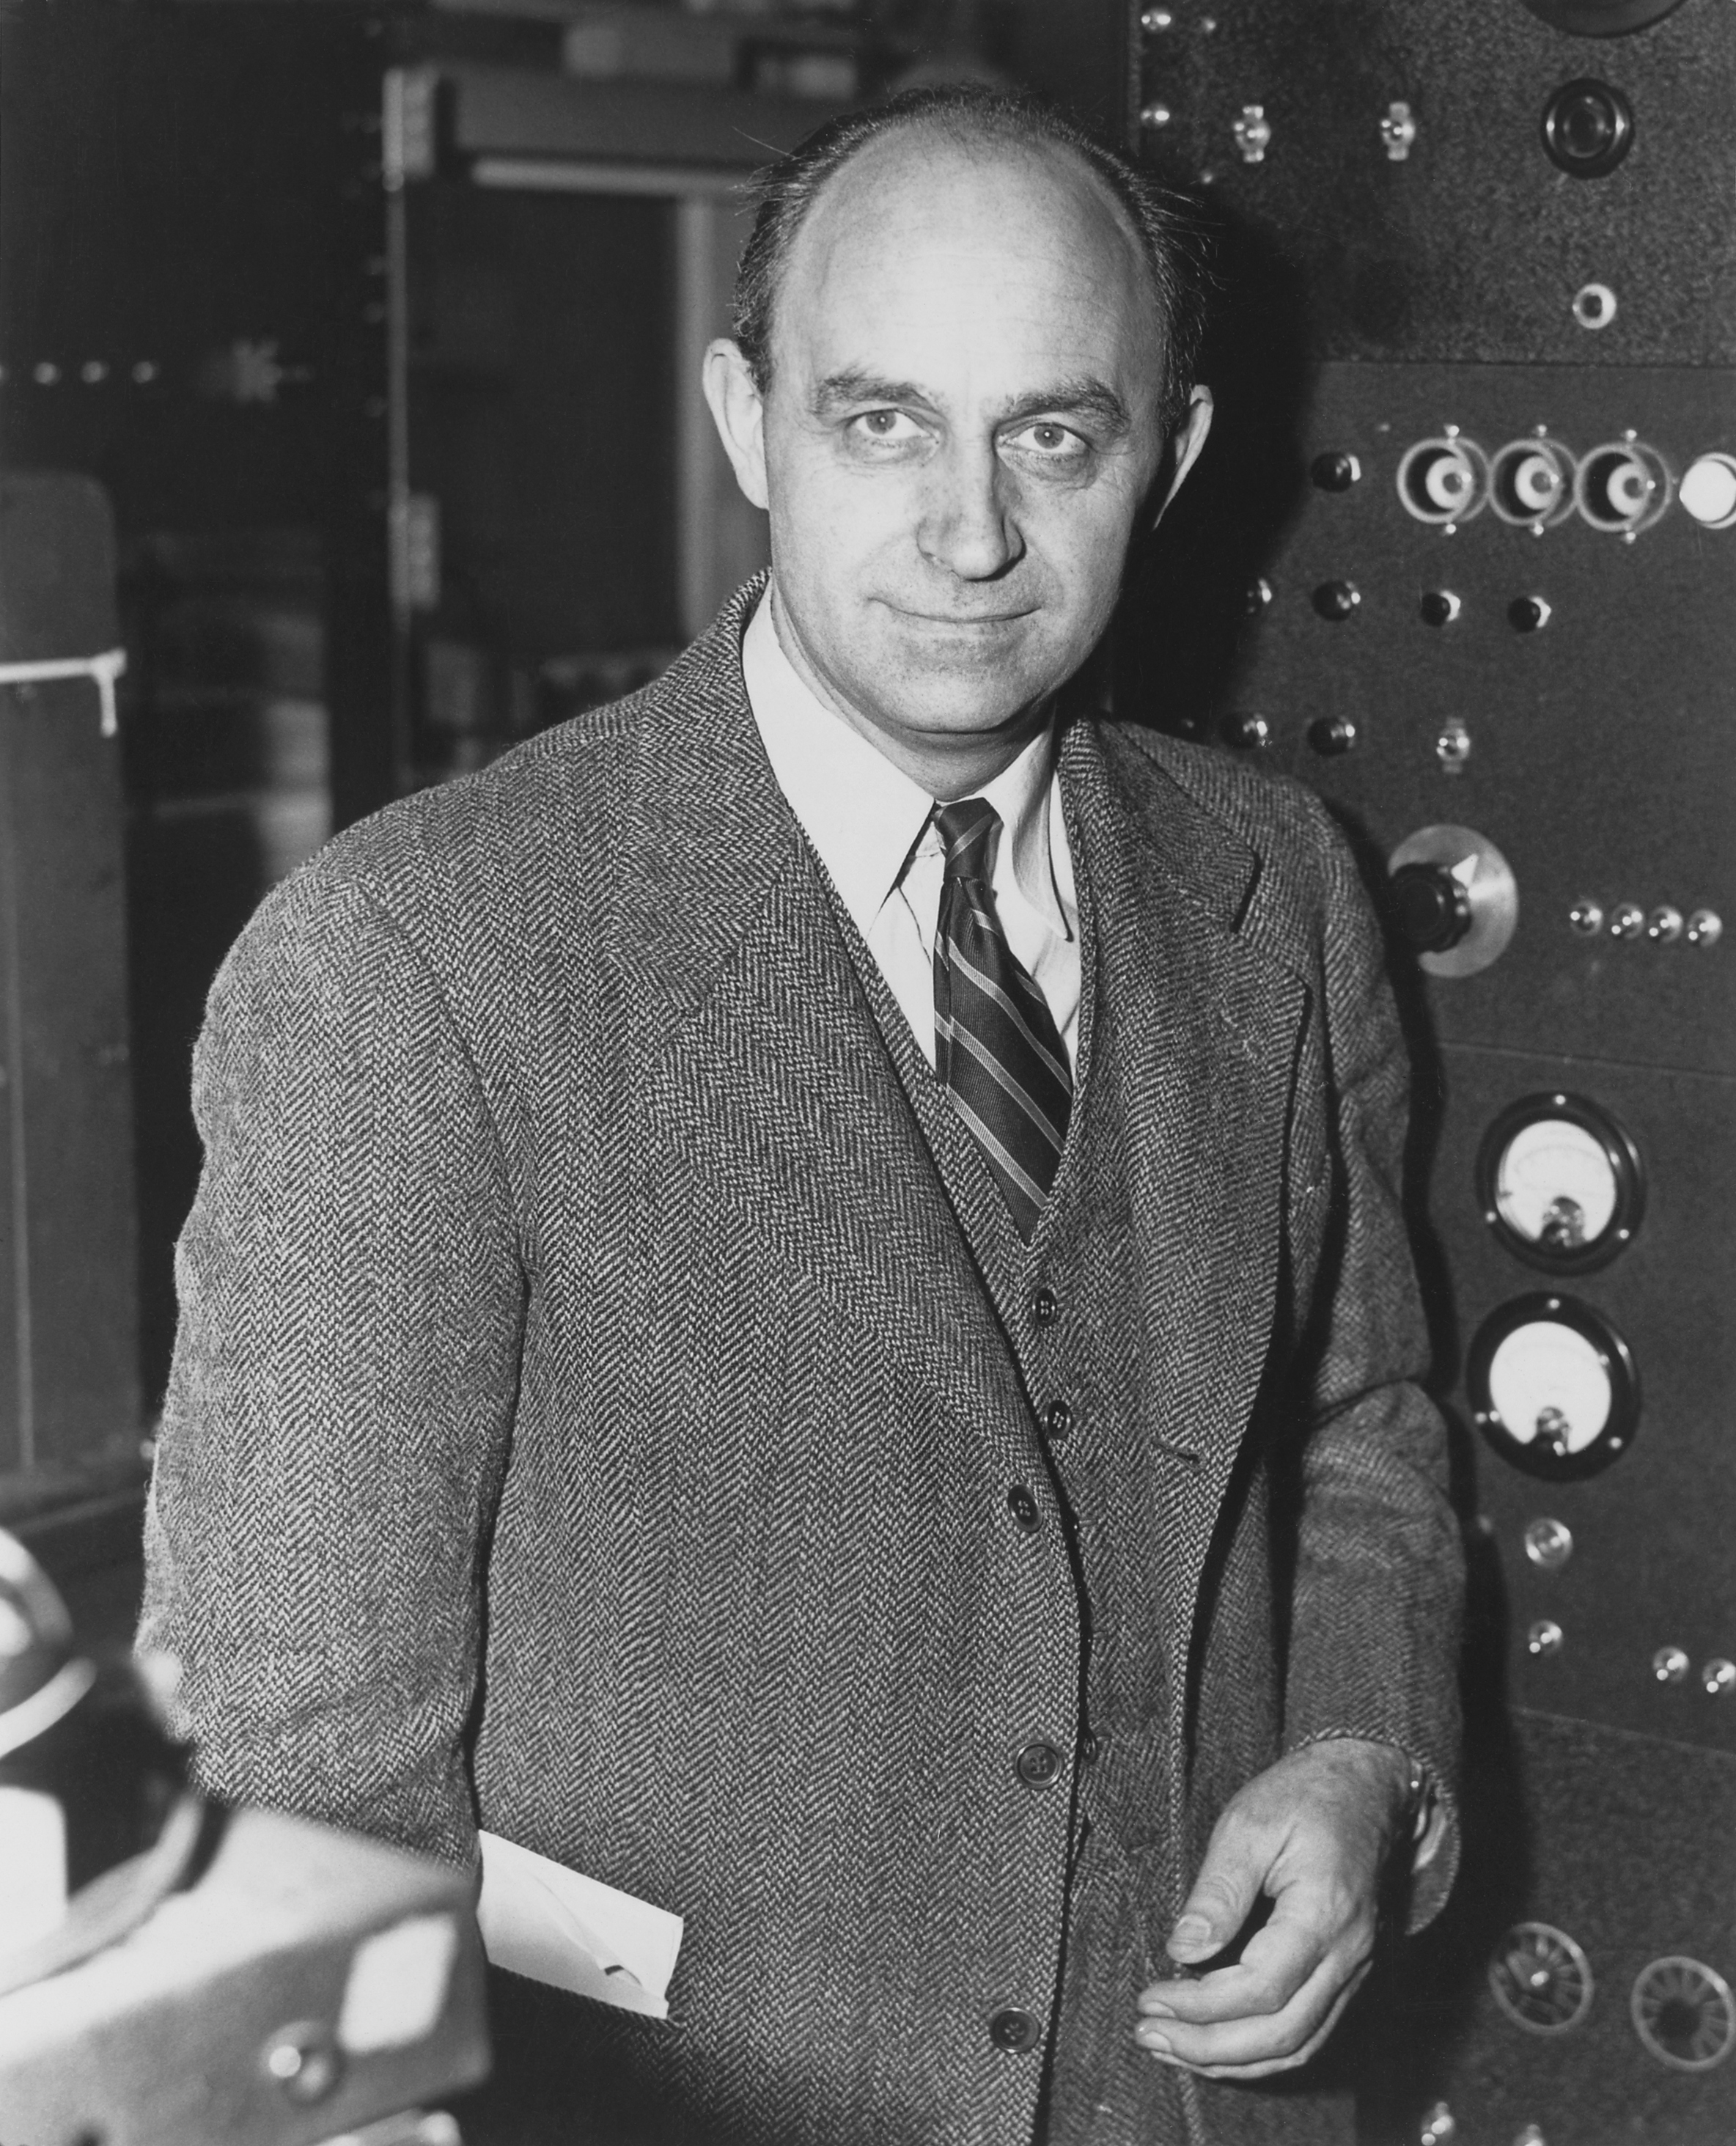
\includegraphics[width=\textwidth]{images/fermi_face.jpg}
            Enrico Fermi
        \end{column}
        
        \begin{column}{0.24\textwidth}
            \centering
            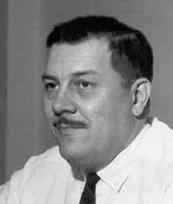
\includegraphics[width=\textwidth]{images/john_pasta.jpg}
            John Pasta
        \end{column}
        
        \begin{column}{0.24\textwidth}
            \centering
            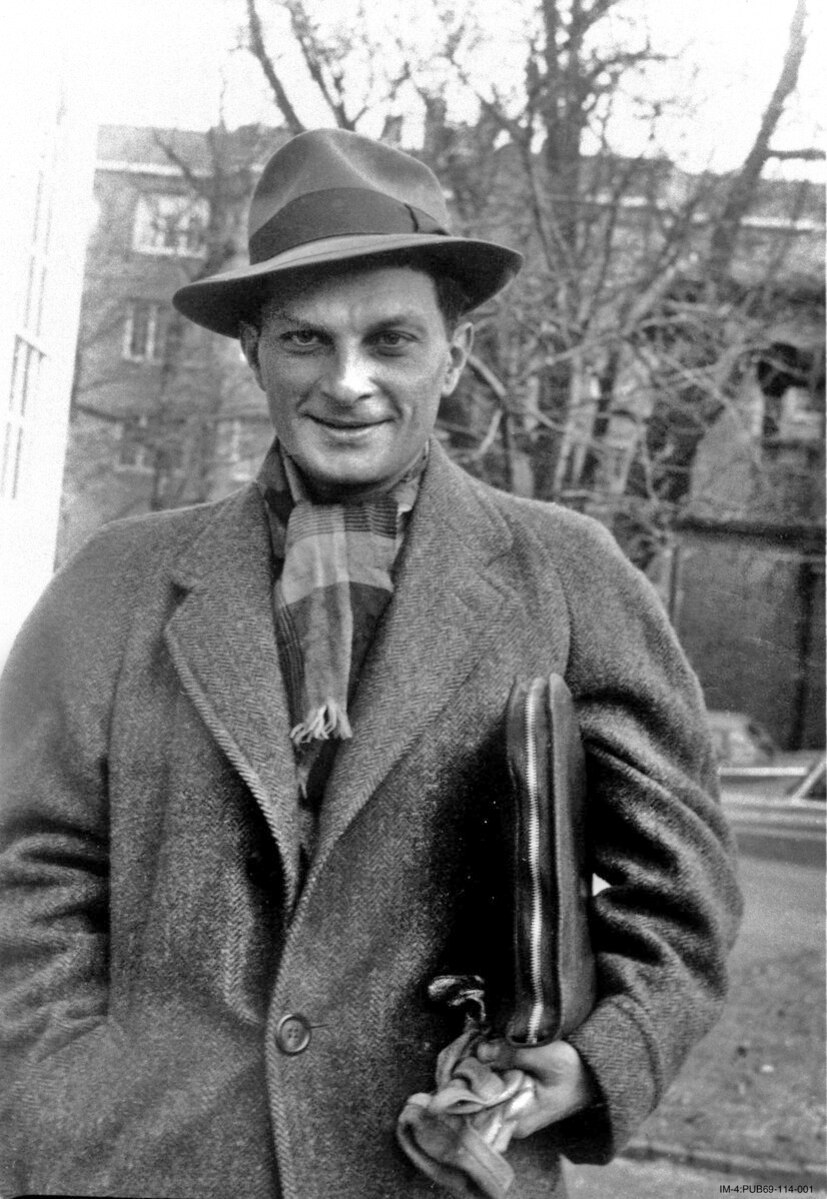
\includegraphics[width=\textwidth]{images/ulam.jpg}
            Stanislaw Ulam
        \end{column}
        
        \begin{column}{0.24\textwidth}
            \centering
            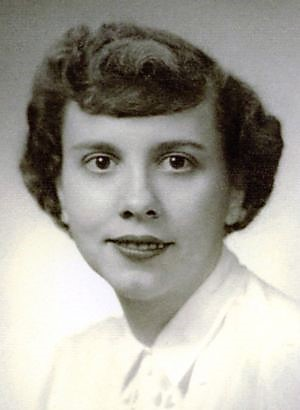
\includegraphics[width=\textwidth]{images/tsingou.jpg}
            Mary Tsingou
        \end{column}
    \end{columns}
\end{frame}


\begin{frame}{FPU Problem Graph}
    \begin{figure}
        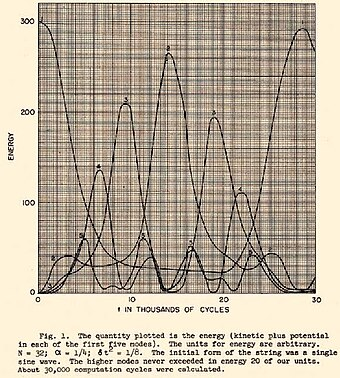
\includegraphics[width=0.5\textwidth]{images/MANIAC.png}
        \caption{Energy vs. time for one of the first N-body systems simulated by Fermi, showing unexpected and non-irreversible behavior.}
    \end{figure}
\end{frame}

\begin{frame}{Towards Realistic Matter Simulations}
    \footnotesize
    With the advent of more powerful computers, simulations became more realistic:
    \pause
    
    \begin{itemize}
        \item \textbf{1957:} Alder and Wainwright simulated elastic collisions between hard spheres using an IBM 704 computer.
        \pause
        \bigskip
        \item \textbf{1960:} Gibson and his team performed perhaps the first realistic simulation, modeling radiation damage in solid copper.
        \pause
        \bigskip
        \item \textbf{1964:} Rahman simulated liquid argon using a \textbf{Lennard-Jones potential}, with results that agreed well with experimental data.
    \end{itemize}
    \pause
    
    \begin{alertblock}<4->{The Legacy of the Lennard-Jones Potential}
        Today, it remains one of the most widely used potentials for describing simple substances and as a component of more complex force fields.
    \end{alertblock}
\end{frame}

\begin{frame}{The Molecular Dynamics Algorithm: Key Steps}
    \begin{block}{Algorithm Steps}
        \begin{enumerate}
            \item \textbf{Initialization:} Initial positions and velocities are assigned to the atoms.
            \pause
            \item \textbf{Force Calculation:} The forces on each atom are calculated, either from classical ($F = -\nabla V(\vec{r})$) or quantum ($F = F(\Psi(\vec{r}))$) potentials.
            \pause
            \item \textbf{Integration:} Positions and velocities are updated for a small time step ($\Delta t$) using an integrator.
            \pause
            \item \textbf{Iteration:} Steps 2 and 3 are repeated for the time required to observe the system's evolution.
        \end{enumerate}
    \end{block}
\end{frame}

\begin{frame}{MD Algorithm Graph}
    \begin{figure}
        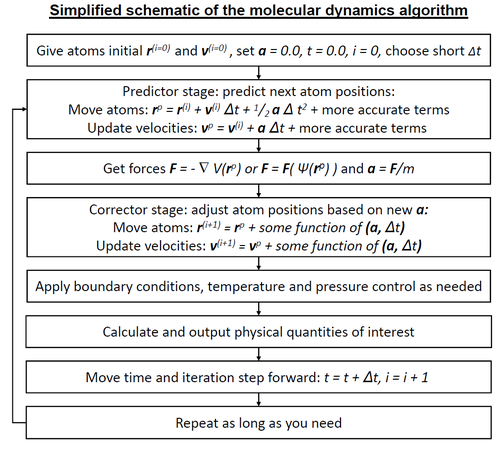
\includegraphics[width=0.5\textwidth]{images/algorithm.png}
        \caption{Simplified schematic of the Molecular Dynamics algorithm.}
    \end{figure}
\end{frame}

% --- START OF THE NEW SECTION ---

\begin{frame}{From Classical to Quantum MD}
    Let's recall the key step in the MD algorithm:
    \pause
    \begin{center}
        \large \textbf{Calculate the Forces}
    \end{center}
    \pause
    
    \begin{itemize}
        \item In classical MD, forces come from \textbf{predefined potentials} (force fields) like the Lennard-Jones potential.
        \pause
        \bigskip
        \item These potentials are efficient, but they \textbf{cannot describe} quantum phenomena like the formation or breaking of chemical bonds, or reactions.
        \pause
        \bigskip
        \item The natural question was: Can we calculate the forces directly from quantum mechanics \textbf{"on the fly"} at each step of the simulation?
    \end{itemize}
    \pause
    
    \begin{alertblock}<6->{The Birth of Quantum Molecular Dynamics}
        This idea gives rise to \textbf{Ab Initio Molecular Dynamics (AIMD)}, where forces are obtained by solving the Schrödinger equation for the electrons at each atomic configuration.
    \end{alertblock}
\end{frame}

%------------------------------------------------

\begin{frame}{The Breakthrough: The Car-Parrinello Method (1985)}
    The field of AIMD was revolutionized by a paper from \textbf{Roberto Car and Michele Parrinello}.
    \pause
    
    \begin{block}{The Car-Parrinello Innovation (CPMD)}
        \begin{itemize}
            \item Instead of fully solving for the electronic state at each step (which is very expensive), they introduced a \textbf{fictitious dynamics} for the electronic orbitals.
            \pause
            \item This unified the evolution of the nuclei (classical) and the electrons (quantum) into a \textbf{single Lagrangian dynamical system}.
            \pause
            \item It allowed for much longer and more efficient simulations than previous methods, opening the door to the study of complex systems in chemistry and materials science.
        \end{itemize}
    \end{block}
    \pause
    
    \begin{exampleblock}<4->{Impact}
        The Car-Parrinello method turned quantum molecular dynamics into a practical and predictive tool, and it remains one of the pillars of the field today.
    \end{exampleblock}
\end{frame}

%------------------------------------------------

\begin{frame}{Two Main Approaches in AIMD}
    From these developments, two main families of Quantum Molecular Dynamics emerged:
    \pause
    
    \begin{columns}
        \begin{column}{0.5\textwidth}
            \begin{block}{Born-Oppenheimer Molecular Dynamics (BOMD)}
                \begin{itemize}
                    \item Strictly adheres to the Born-Oppenheimer approximation.
                    \item \textbf{Calculates the electronic ground state} accurately at each time step.
                    \item It is conceptually simpler and very robust.
                    \item It generally allows for larger time steps, but each step is more computationally expensive.
                \end{itemize}
            \end{block}
        \end{column}
        \begin{column}{0.5\textwidth}
            \begin{block}{Car-Parrinello Molecular Dynamics (CPMD)}
                 \begin{itemize}
                    \item Propagates the nuclei and electronic orbitals simultaneously.
                    \item The electrons are \textbf{not exactly in the ground state} at each step, but they remain close to it.
                    \item It is computationally more efficient per time step.
                    \item It requires smaller time steps to maintain adiabaticity.
                \end{itemize}
            \end{block}
        \end{column}
    \end{columns}
\end{frame}

% --- END OF THE NEW SECTION ---

\begin{frame}{The Classical Limitation and the Quantum Leap}
    Classical potentials like Lennard-Jones are excellent, but they cannot describe processes where electrons are key, such as:
    \pause
    \begin{itemize}
        \item Bond formation and breaking.
        \item Chemical reactions.
        \item Electronic properties and polarization.
    \end{itemize}
    \pause
    \bigskip
    
    \begin{block}{The Quantum Need}
        To simulate these phenomena, forces on the atoms must be calculated from the system's electronic structure using quantum mechanics. This gives rise to \textbf{Quantum Molecular Dynamics (QMD)} or \textbf{Ab Initio Molecular Dynamics (AIMD)}.
    \end{block}
\end{frame}


% --- SECTION 2: History of DFT ---
\section{History of Density Functional Theory (DFT)}

\begin{frame}{\large I. Origins: The Precursors}
    \framesubtitle{The Density as a Basic Variable}
    \begin{itemize}
        \item The earliest density-based methods trace back to the Thomas, Fermi, and Dirac papers (1927–1930).
        \item \textbf{The Thomas-Fermi-Dirac model} described atoms based purely on the electron density $n(\mathbf{r})$.
        \item The motivation was to find "approximate practical methods" to solve the complicated quantum mechanical equations (Dirac, 1929).
        \item Limitation: The Thomas-Fermi model has severe deficiencies, such as the inability to predict molecular or solid binding.
    \end{itemize}
\end{frame}

% 4. Modern Formalism
\begin{frame}{\large II. Modern Density Functional Formalism (HK)}
    \framesubtitle{The Hohenberg-Kohn Theorems (1964)}
    \begin{itemize}
        \item HK Theorem 1: The external potential $V_{\text{ext}}(\mathbf{r})$ (and thus the full Hamiltonian) is uniquely determined by the ground-state electron density $n(\mathbf{r})$.
        \item HK Theorem 2: A universal functional for the energy, $E[n]$, exists, and the correct ground-state density minimizes this Functional.
        \begin{equation*}
            E[n, V_{\text{ext}}] = F[n] + \int n(\mathbf{r}) V_{\text{ext}}(\mathbf{r}) d\mathbf{r} \quad (\text{Variational Principle})
        \end{equation*}
        \item This formal grounding eliminated the need for the complicated $3N$-dimensional wave function $\Psi(\mathbf{r}_1, \ldots, \mathbf{r}_N)$.
    \end{itemize}
\end{frame}

% 5. The KS Scheme
\begin{frame}{\large III. The Kohn-Sham Scheme and Approximations}
    \framesubtitle{The Practical Method (1965)}
    \begin{itemize}
        \item The Kohn-Sham (KS) scheme introduced a non-interacting auxiliary system that produces the exact ground-state density $n(\mathbf{r})$ of the real interacting system.
        \item This turns the many-body problem into a set of solvable single-particle equations (Kohn-Sham equations).
        \item The complexity is now contained in the exchange-correlation functional $E_{xc}[n]$.
        \item Key Approximations:
        \begin{itemize}
            \item Local Density Approximation (LDA): Based on the homogeneous electron gas.
            \item Generalized Gradient Approximation (GGA): Introduced dependence on the density gradient, $\nabla n$.
        \end{itemize}
    \end{itemize}
\end{frame}

% -------------------------
\section{Rise to Prominence}
% -------------------------

% 6. The Breakthrough (1990-Present)
\begin{frame}{\large IV. The Rise to Prominence (Post-1990)}
    \begin{itemize}
        \item Widespread application, particularly in chemistry and materials science, grew astonishingly after 1990.
        \item The number of publications citing DFT/DF increased dramatically, marking a huge success story (Fig. 1).
        \item Crucial Developments:
        \begin{itemize}
            \item Car-Parrinello Molecular Dynamics (1985): Combined DFT with MD, enabling efficient study of structures and reactions.
            \item Improved Functionals: Development of GGAs and hybrid functionals (e.g., incorporating Hartree-Fock exact exchange).
        \end{itemize}
        \item A 1991 conference in Menton is cited as a major turning point for acceptance among chemists.
    \end{itemize}
\end{frame}

% 7. Current Successes
\begin{frame}{\large V. Current Status and Applications}
    \framesubtitle{A Standard Tool in Modern Science}
    \begin{itemize}
        \item DFT is now well-established in condensed matter physics and has a significant presence in theoretical chemistry.
        \item It is particularly valuable for calculating the total energy ($E$) and energy surfaces $E(\mathbf{R}_i)$, which are essential for determining ground-state structures and chemical reaction paths.
        \item DFT allows calculations of complex systems in biochemistry and materials science that were "far beyond expectations" in 1990.
    \end{itemize}
\end{frame}

% -------------------------
\section{Challenges and Future}
% -------------------------

% 8. Future and Challenges
\begin{frame}{\large VI. Challenges and Future Outlook}
    \framesubtitle{Quo Vadis? (Whither Goest Thou?)}
    \begin{itemize}
        [cite_start]\item Despite its success, prominent practitioners have raised concerns about the future ("best of times and the worst of times")[cite: 209, 210].
        [cite_start]\item **The Central Problem:** The lack of a systematic way to improve the **Exchange-Correlation functional ($E_{xc}$)**[cite: 11, 211].
        \item **Current Challenges:**
        \begin{itemize}
            [cite_start]\item Accurately describing **Dispersion (van der Waals) interactions**[cite: 11].
            [cite_start]\item Treating **"Strongly correlated" systems**[cite: 11].
            [cite_start]\item The proliferation of hundreds of approximate functionals makes choosing the "best" one ambiguous and risks a "semi-empirical" view of the theory[cite: 153, 213].
        \end{itemize}
        [cite_start]\item The field is continually exploring extensions, such as combining DFT with Density Matrix Functional Theory (DMFT) or Quantum Monte Carlo (QMC)[cite: 11, 166].
    \end{itemize}
\end{frame}

% 9. Conclusion
\begin{frame}{\large VII. Conclusion}
    \begin{itemize}
        \item DFT is a huge success story, having moved from theoretical origins to a mainstream computational tool due to the work of Hohenberg, Kohn, and Sham and the subsequent development of reliable functional approximations.
        \item Its widespread acceptance came after 1990, driven by its efficiency and ability to handle large systems, a goal anticipated by Dirac in 1929.
        \item The future of DFT rests on the continuing development of accurate, universal, and physically sound exchange-correlation functionals.
    \end{itemize}
\end{frame}


% --- SECTION 3: Methods of QMD ---
\section{Methods of QMD}
\begin{frame}{Methods for Electronic Dynamics}{By Propagation Algorithm}
    \textbf{Born-Oppenheimer Molecular Dynamics (BOMD)}
    \vspace{1em}
    
    \textbf{Car-Parrinello Molecular Dynamics (CPMD)}
    \vspace{1em}
    
    \textbf{Ehrenfest Molecular Dynamics}
\end{frame}

\begin{frame}{Methods for Electronic Dynamics}{By Level of Electronic Theory}
    \begin{block}{Density Functional Theory (DFT-MD)}
    \end{block}
    
    \begin{block}{Wavefunction Theory (WFT-MD)}
        \textbf{Hartree-Fock (HF-MD)}
        \vspace{0.5em}
        
        \textbf{Post-Hartree-Fock (MP2-MD, CCSD-MD)}
    \end{block}
    
    \begin{block}{Semi-empirical Methods (SE-MD)}
    	\textbf{MNDO - Modified Neglect of Diatomic Overlap}
    \end{block}
\end{frame}

\subsection{Semi-Epirical (MNDO, AM1, Tight-Bending)}

%-----------------MNDO----------------------------

\begin{frame}{MNDO}
	\begin{block}{Paper Title}
	Ground State of Molecules The MNDO Method Approximation and Parameters
	\end{block}
\end{frame}

\begin{frame}{The MNDO method}
    \begin{block}{Objective}
        To develop a fast and reliable quantum method for predicting molecular properties.
    \end{block}
    \pause
    
    \begin{itemize}
        \item It is a \textbf{semiempirical} method, meaning it combines theory with experimental parameters.
        \pause
        \bigskip
        \item Its theoretical basis is the \textbf{NDDO} (Neglect of Diatomic Differential Overlap) approximation, which is more rigorous than previous methods like INDO or CNDO.
    \end{itemize}
\end{frame}



\begin{frame}{Approximation I: One-Center Terms}
    \begin{block}{Energies and Repulsions on a Single Atom}
        \begin{itemize}
            \item The terms that describe the energy of an electron in an atom ($U_{\mu\mu}$) and the repulsion between electrons on the same atom ($g_{\mu\nu}$, $h_{\mu\nu}$) are not calculated theoretically.
            \pause
            \bigskip
            \item Instead, they are derived by fitting the calculations to \textbf{experimental spectroscopic data} for the atom and its ions.
            \pause
            \bigskip
            \item This implicitly introduces an \textbf{electron correlation} effect, as the fitted values are smaller than the theoretical ones.
        \end{itemize}
    \end{block}
\end{frame}



\begin{frame}{Approximation II: Two-Center Repulsion}
    \begin{alertblock}{The Key Innovation of MNDO}
        The repulsion between the charge distribution of an atom A and another atom B is modeled classically.
    \end{alertblock}
    \pause
    
    \begin{itemize}
        \item The interaction is decomposed into a sum of interactions between \textbf{multipoles} (monopole, dipole, quadrupole).
        \pause
        \bigskip
        \item Each multipole is in turn represented as a simple configuration of \textbf{point charges}.
        \pause
        \bigskip
        \item The final repulsion energy is calculated by summing the interactions between these point charges using a semiempirical formula.
    \end{itemize}
\end{frame}



\begin{frame}{Approximation III: Chemical Bonding}
    \begin{block}{Core-Core and Resonance Interactions}
        \begin{itemize}
            \item \textbf{Core-Core Repulsion:} The repulsion between the nuclei and inner-shell electrons ("cores") is modeled with a function that blends charge repulsion with an adjustable exponential term.
            \pause
            \bigskip
            \item \textbf{Resonance Integrals ($\beta_{\mu\lambda}$):} These are responsible for most of the bonding energy. They are assumed to be proportional to the overlap of the atomic orbitals, with a constant that depends on atomic parameters.
        \end{itemize}
    \end{block}
\end{frame}



\begin{frame}{The Parametrization Process}
    \begin{block}{Fitting to Experimental Reality}
        \begin{itemize}
            \item The mathematical expressions in the method contain a series of \textbf{atomic parameters} ($\zeta, U_{ss}, \beta_p$, etc.).
            \pause
            \bigskip
            \item The values of these parameters are not derived from theory. They are obtained through a \textbf{nonlinear least-squares optimization process}.
            \pause
            \bigskip
            \item The parameters are adjusted until the calculated properties (heats of formation, geometries, etc.) for a set of standard molecules match their \textbf{experimental values} as closely as possible.
        \end{itemize}
    \end{block}
\end{frame}

%-------------AM1------------------------------------------

\begin{frame}{AM1}
	\begin{block}{Paper Title}
	AM1: A New Method General Purpose Quantum Mechanical Molecular Model
	\end{block}
\end{frame}

\begin{frame}
  \frametitle{AM1 - Austin Model 1}
  
  \begin{itemize}
    \item \textbf{Austin Model 1 (AM1)} is a semiempirical quantum mechanical molecular model developed in the mid-80s by Michael J. S. Dewar's group. \pause
    \item \textbf{Objective:} To be a general-purpose computational tool for studying: \pause
    \begin{itemize}
        \item Large molecular systems. \pause
        \item Chemical reactions and their mechanisms. \pause
    \end{itemize}
    \item It was created as an alternative to \textit{ab initio} methods, which were prohibitively expensive in terms of computation time for molecules of real chemical interest.
  \end{itemize}
\end{frame}

\begin{frame}
  \frametitle{The Predecessor: Weaknesses of MNDO}
  
  AM1 is a direct evolution of the MNDO (\textit{Modified Neglect of Diatomic Overlap}) method and was designed to correct its most significant flaws: \pause
  
  \begin{block}{Main Flaws of MNDO}
    \begin{itemize}
      \item Inability to correctly reproduce \textbf{hydrogen bonds}. \pause
      \item Overestimation of interatomic repulsions, leading to errors in: \pause
      \begin{itemize}
          \item Sterically hindered molecules (e.g., neopentane). \pause
          \item Molecules with four-membered rings. \pause
      \end{itemize}
      \item A tendency to calculate activation energies that were too high.
    \end{itemize}
  \end{block}
\end{frame}


\begin{frame}
  \frametitle{Methodology and Key Improvements}
  
  \begin{itemize}
    \item AM1 is based on the same approximation as MNDO: \textbf{Neglect of Diatomic Differential Overlap (NDDO)}. \pause
    \item \textbf{Key Modification:} The \textbf{Core Repulsion Function (CRF)} was optimized. \pause
    \begin{itemize}
        \item \textbf{Gaussian terms} were added to the MNDO function. \pause
        \item This allows for the adjustment of interatomic repulsions to improve the description of medium and long-range interactions. \pause
    \end{itemize}
    \item The parameters for the elements C, H, O, and N were optimized simultaneously, using a larger dataset and an improved optimization procedure.
  \end{itemize}
\end{frame}

% --- Slide on Results and Advantages ---
\begin{frame}
  \frametitle{Results and Advantages of AM1}
  
  AM1 proved to be a substantial improvement over MNDO without increasing computation time. \pause
  
  \begin{alertblock}{Main Advantages}
    \begin{itemize}
      \item<2-> Capable of genuinely modeling \textbf{hydrogen bonds}. \pause
      \item<3-> More accurate estimates of \textbf{activation energies}. \pause
      \item<4-> Better treatment of \textbf{hindered molecules} (e.g., neopentane) and those with ring strain (e.g., cubane).
    \end{itemize}
  \end{alertblock}
  
\end{frame}

%------------------------Tight-Bending---------------------

\begin{frame}{Tight-Bending}
	\begin{block}{Paper Title}
	Self-consistent-charge density-functional tight-binding method for simulations of complex
materials properties
	\end{block}
\end{frame}

\begin{frame}
  \frametitle{The Limits of Standard Tight-Binding}
  
  Standard Tight-Binding (TB) is a computationally fast method derived from Density-Functional Theory (DFT). \pause
  
  \begin{itemize}
    \item It works well when the charge density of a system can be approximated as a simple superposition of neutral atom densities. \pause
    
    \item However, it has a significant limitation: it is a \textbf{non-self-consistent} method. \pause
    
    \item This means it cannot account for the transfer of charge between different types of atoms. This leads to failures in polar or heteronuclear systems and limits the method's overall transferability.
  \end{itemize}
\end{frame}

\begin{frame}
  \frametitle{The SCC-DFTB Solution: Self-Consistent Charges}
  
  The Self-Consistent-Charge (SCC) method extends the standard approach by allowing the system's charges to re-distribute. \pause
  
  \begin{block}{The Core Principle}
    It is based on a second-order expansion of the DFT total energy with respect to fluctuations in the charge density ($\delta n$).
  \end{block} \pause
  
  \begin{itemize}
    \item A new energy term is added that depends on the Mulliken charge fluctuations ($\Delta q$) on each atom. \pause
    
    \item This term correctly describes long-range Coulomb interactions between charges and includes on-site self-interaction effects related to an atom's chemical hardness (the Hubbard parameter U). \pause
    
    \item The method then iterates, adjusting the charges and recalculating the energy until a self-consistent, minimum-energy solution is found.
  \end{itemize}
\end{frame}

\begin{frame}
  \frametitle{Why It Matters: The Payoff of SCC-DFTB}
  
  This self-consistent charge correction makes the method significantly more accurate and robust. \pause
  
  \begin{alertblock}{Key Advantages}
    \begin{itemize}
      \item \textbf{Enhanced Transferability:} By properly treating charge transfer, the method is successfully applied to a much broader range of systems, including polar molecules, semiconductors, and large biomolecules. \pause
      
      \item \textbf{Improved Accuracy:} It leads to a considerable improvement in total energies, forces, vibrational frequencies, and molecular geometries compared to the non-SCC approach. \pause
      
      \item \textbf{Efficiency is Maintained:} The self-consistent cycle is very fast, typically converging in just 3-5 iterations. The method remains orders of magnitude faster than ab initio calculations.
    \end{itemize}
  \end{alertblock}
  
\end{frame}

\subsection{Post-Hartree-Fock (MP2-MD, CCSD-MD)}

%--------------------------CCSD------------------

\begin{frame}{CCSD-MD}
	\begin{block}{Paper Title}
	On the Correlation Problem in Atomic and Molecular Systems. Calculation of Wavefunction Components in Ursell-Type Expansion Using Quantum Field Theoretical Methods 
	\end{block}
\end{frame}


\begin{frame}{Coupled Cluster (CC) Method}
    \begin{block}{The Problem: Electron Correlation}
        Standard methods like Hartree-Fock ignore that electron movements are correlated. The CC method aims to calculate this \textbf{correlation energy}.
    \end{block}
    \pause

    \begin{alertblock}{The Central Idea: The Exponential Ansatz}
        It expresses the exact wavefunction $|\Psi\rangle$ by applying an exponential "cluster operator" $e^{\hat{T}}$ to the Hartree-Fock wavefunction $|\Phi\rangle$:
        \[
        |\Psi\rangle = e^{\hat{T}} |\Phi\rangle
        \]
    \end{alertblock}
\end{frame}

%------------------------------------------------

\begin{frame}{How Coupled Cluster Works}
    \begin{itemize}
        \item The \textbf{cluster operator} $\hat{T}$ is a sum of excitation operators ($\hat{T} = \hat{T}_1 + \hat{T}_2 + \dots$), where $\hat{T}_1$ creates single excitations, $\hat{T}_2$ creates double excitations, and so on.
        \pause
        \bigskip
        \item The method uses tools from \textbf{quantum field theory} (hole-particle formalism, Wick's theorem) to solve for the amplitudes of these excitations.
        \pause
        \bigskip
        \item Its key advantage over Configuration Interaction (CI) is that truncating at $\hat{T}_2$ (CCSD) still includes the most important effects of quadruple excitations, making the method very efficient and \textbf{size-extensive}.
    \end{itemize}
\end{frame}

\begin{frame}{CCSD vs GCCSD}
    \begin{figure}
        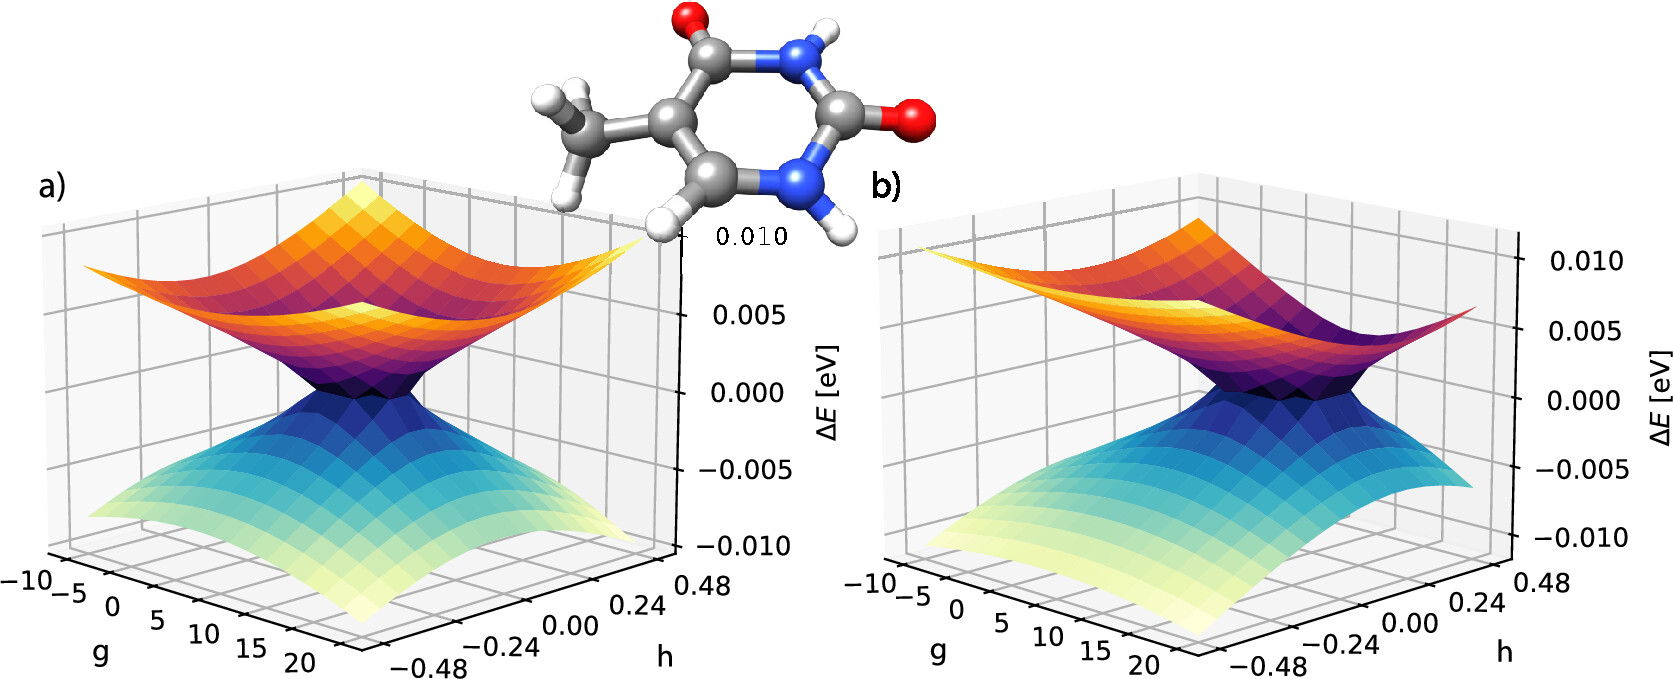
\includegraphics[width=0.8\textwidth]{images/CCSD.jpeg}
        \caption{Superficies de energía potencial S1 y S2 en timina calculadas con CCSD (a) y GCCSD (b).}
    \end{figure}
\end{frame}

\begin{frame}{Methods for Non-Adiabatic Dynamics}
    \textbf{Trajectory Surface Hopping (TSH)}
    \vspace{1.5em}
    
    \textbf{Multi-Configuration Time-Dependent Hartree (MCTDH)}
\end{frame}
\begin{frame}{Methods Including Nuclear Quantum Effects}
    \textbf{Path Integral Molecular Dynamics (PIMD)}
    \begin{itemize}
        \item Centroid Molecular Dynamics (CMD)
        \item Ring Polymer Molecular Dynamics (RPMD)
    \end{itemize}
    \vspace{1em}

    \textbf{Wave Packet Propagation}
\end{frame}

\subsection{PIMD}

%---------------------PIMD------------------------------------------

\begin{frame}{PIMD (Path Integral Molecular Dynamics)}
	\begin{block}{Paper Title}
	Study of an F center in molten KCl
	\end{block}
\end{frame}

\begin{frame}
  \frametitle{The Problem: A Quantum Particle in a Classical World}
  
  Simulating systems with both quantum and classical particles presents a major challenge. \pause
  
  \begin{itemize}
    \item Consider an electron (a quantum particle) dissolved in a bath of classical ions, like molten salt. \pause
    
    \item The electron does not have a fixed position; its quantum nature means it is "fuzzy" and delocalized. \pause
    
    \item How can we combine the quantum statistical mechanics of the electron with the classical statistical physics of the ions in a single simulation?
  \end{itemize}
\end{frame}

\begin{frame}
  \frametitle{The Path Integral Solution: A Quantum-Classical Isomorphism}
  
  The method uses Richard Feynman's path integral formulation to map the quantum problem onto an equivalent classical problem. \pause
  
  \begin{block}{The Isomorphism}
    A single quantum particle is formally proven to be equivalent to a classical \textbf{ring polymer} (or "necklace") made of P beads.
  \end{block} \pause
  
  \begin{itemize}
    \item Each bead in the necklace is connected to its two neighbors by \textbf{harmonic springs}. This part of the model represents the quantum kinetic energy. \pause
    
    \item Every bead also interacts with the external potential created by the classical particles. \pause
    
    \item This mapping becomes exact as the number of beads (P) approaches infinity. In practice, a finite but sufficiently large P is used.
  \end{itemize}
\end{frame}

\begin{frame}
  \frametitle{Simulating the Necklace: PIMD in Action}
  
  Once the quantum particle is represented as a classical polymer, the entire system can be simulated using standard \textbf{Molecular Dynamics (MD)}. \pause
  
  \begin{alertblock}{Physical Interpretation}
    \begin{itemize}
      \item The \textbf{spatial spread} of the polymer beads directly represents the quantum "fuzziness" or delocalization of the particle. \pause
      \begin{itemize}
          \item A compact, collapsed necklace means the particle is highly localized (like an F center).
          \item A spread-out, large necklace means the particle is delocalized. \pause
      \end{itemize}
      \item This allows us to calculate quantum properties like kinetic energy and study phenomena like electron localization, all within a classical simulation framework.
    \end{itemize}
  \end{alertblock}
  
\end{frame}

%-----------------CMD---------------------------------------------

\begin{frame}{CMD (centroid molecular dynamics)}
	\begin{block}{Paper Title}
	The formulation of quantum statistical mechanics based on the Feynman path
centroid density. II. Dynamical properties
	\end{block}
\end{frame}

\begin{frame}
  \frametitle{Beyond Static Properties: The Challenge of Quantum Dynamics}
  
  The Path Integral formalism (PIMD) is excellent for calculating equilibrium quantum properties by mapping a particle to a classical ring polymer. \pause
  
  \begin{itemize}
    \item However, the "dynamics" used in a PIMD simulation are fictitious; they are simply a tool to sample configurations. \pause
    
    \item This leaves a critical question open: How can we calculate \textbf{real-time dynamical properties}, such as time correlation functions $\langle A(t)B(0)\rangle$? \pause
    
    \item We need a way to extract real physical evolution from the path integral framework.
  \end{itemize}
\end{frame}

\begin{frame}
  \frametitle{Centroid Molecular Dynamics (CMD): The Core Idea}
  
  The CMD method proposes that the most important dynamical information is captured by a special variable: the \textbf{path centroid}. \pause
  
  \begin{itemize}
    \item The centroid is the center of mass (average position) of all the beads in the path integral polymer. It is considered the most direct classical-like variable in the quantum system. \pause
    
    \item \textbf{The Central Approximation:} The full, complex quantum dynamics of a particle can be effectively approximated by the \textbf{classical evolution of its centroid}. \pause
    
    \item However, the centroid does not move on the classical potential. It evolves on a \textbf{quantum potential of mean force} ($V_c$). \pause
    
    \item This "centroid potential" is an effective potential averaged over all the quantum fluctuations of the polymer beads, and it implicitly includes quantum effects like zero-point energy and tunneling.
  \end{itemize}
\end{frame}

\begin{frame}
  \frametitle{CMD in Action: A "Quasiclassical" Simulation}
  
  The CMD method provides a practical algorithm for simulating quantum dynamics. \pause
  
  \begin{block}{The Simulation Process}
    A molecular dynamics simulation is performed, but only for the centroid coordinates, which behave like classical particles.
  \end{block} \pause
  
  \begin{itemize}
    \item These centroids evolve according to Newton's equations of motion ($F_c = m \ddot{q}_c$). \pause
    
    \item The force ($F_c$) is not the classical force, but the \textbf{quantum mean force}, derived from the gradient of the centroid potential ($F_c = -\nabla V_c$). \pause
    
    \item The resulting "centroid trajectories" are then used to compute approximate quantum time correlation functions. \pause
  \end{itemize}
  
  \begin{alertblock}{Key Advantage}
    The computational cost of a CMD simulation scales in the same way as a purely classical simulation, making it a powerful tool for studying quantum dynamical effects in large, complex systems.
  \end{alertblock}
\end{frame}
=======
\begin{frame}{RPMD for Real-Time Quantum Correlation Functions}

\begin{itemize}
    \item \textbf{The Problem:} The exact calculation of quantum real-time correlation functions is still considered "a very difficult problem".
    
    \item \textbf{General Approach:} A number of methods have been proposed to include short-time quantum mechanical effects in classical molecular dynamics simulations. These methods typically combine an exact treatment of the quantum Boltzmann operator with an approximate treatment of the real-time evolution based on classical mechanics.
    
    \item \textbf{The Proposed Method (RPMD):} We propose an approximate method, based on path integral (Parrinello-Rahman) molecular dynamics, for calculating \textbf{Kubo-transformed real-time correlation functions} involving position-dependent operators.
    
    \item \textbf{Core Idea:} Exploit the isomorphism between the path integral representation of the quantum mechanical partition function and the classical partition function of a fictitious ring polymer.
\end{itemize}
\end{frame}

\begin{frame}{Methodology: Kubo Transform and Dynamics}

\begin{itemize}
    \item \textbf{Object of Interest:} The method focuses on the Kubo-transformed correlation function, $\tilde{C}_{AB}(t)$.
    \begin{itemize}
        \item This function is appealing because it has the same symmetries as a classical correlation function.
    \end{itemize}

    \item \textbf{Initial Condition ($t=0$):} The $t \to 0$ limit of $\tilde{C}_{AB}(t)$ coincides with a purely classical phase space average $\langle A_n(x) B_n(x) \rangle_n$ calculated for the fictitious ring polymer system.
\end{frame}
	\begin{frame}
    \item \textbf{Time Evolution:} To extend this result to times $t > 0$, the method uses the classical dynamics generated by the ring polymer Hamiltonian $H_n(p,x)$.
    \begin{itemize}
        \item The resulting correlation function, $\langle A(0)B(t) \rangle_n$, is calculated via integration over initial phase space variables evolved using the classical equations of motion.
    \end{itemize}
    
    \item \textbf{Symmetry Guarantee:} The classical ring-polymer correlation function $\langle A(0)B(t) \rangle_n$ maintains the crucial symmetries of $\tilde{C}_{AB}(t)$, including the quantum mechanical detailed balance condition.
\end{itemize}
\end{frame}

\begin{frame}{Key Analytical Results and Advantages}

\begin{itemize}
    \item \textbf{RPMD is Exact at $t=0$:} The resulting correlation functions coincide with the exact quantum mechanical result in the limit as $t \to 0$ (for sufficiently large $n$).
    
    \item \textbf{The Harmonic Limit:} RPMD gives the exact quantum mechanical result $\tilde{C}_{AB}(t)$ for all times $t$ in a harmonic potential, provided that one or both operators ($A(\hat{x})$ or $B(\hat{x})$) are linear functions of position.
    \begin{itemize}
        \item For the position autocorrelation function $\tilde{C}_{xx}(t)$, the classical limit ($n=1$ polymer bead) is already exact in the harmonic case.
    \end{itemize}
    
    \item \textbf{Consistent Improvement:} The RPMD correlation functions are consistently better than those given by purely classical molecular dynamics.
    \begin{itemize}
        \item This improvement is \textbf{most apparent in the low-temperature regime} where quantum statistics are critically important.
    \end{itemize}
    
    \item \textbf{Computational Efficiency:} RPMD requires less computational work compared to the related centroid molecular dynamics method, yet its results are only marginally less accurate for tested problems.
\end{itemize}
\end{frame}

\begin{frame}{Limitations and Summary}

\begin{itemize}
    \item \textbf{Short-Time Focus:} The method is designed primarily to give an accurate approximation to the quantum mechanical correlation function for times on the order of the thermal time ($\beta\hbar$).
    
    \item \textbf{Missing Quantum Dynamics:} The neglect of quantum phase information in the subsequent dynamics is clearly undesirable.
    
    \item \textbf{Failure for Long-Time Coherences:} The method misses long-time quantum coherence effects that arise in simple one-dimensional anharmonic systems (e.g., the quartic oscillator).
    \begin{itemize}
        \item This failure is expected, as the method does not contain the phase information needed to capture long-time quantum oscillations.
        \item The method performs well only in situations where quantum effects in the dynamics are comparatively unimportant.
    \end{itemize}
    
    \item \textbf{Summary:} RPMD successfully includes short-time quantum effects stemming from the Boltzmann operator, providing a consistent improvement over classical MD, especially at lower temperatures.
    
    \item \textbf{Future Work:} It will be interesting to test RPMD in condensed phase applications, such as calculating the infrared absorption spectrum of liquid water.
\end{itemize}
\end{frame}

\begin{frame}{Hybrid Methods}
    \begin{block}{Quantum Mechanics / Molecular Mechanics (QM/MM)}
    \end{block}
\end{frame}




% --- SECTION 4: General Conclusions ---
\section{General Conclusions}
\input{conclusions.tex}

% --- SECTION 5: References ---
\section{References}

\begin{frame}[allowframebreaks]{References}
    % This single command prints the bibliography
    \printbibliography
    \nocite{*}
\end{frame}

\end{document}